Overview words about event selection

\subsection{Exclusivity Cuts}\label{sec:eventselection}

    \begin{wrapfigure}{r}{0.58\textwidth}
    	\vspace*{-0.3cm}
    	\includegraphics[page=10,width=0.97\linewidth]{Chapters/Ch4-BaseAnalysis/1_Event_Selection_Cuts/figures/eppi0.exclusive.pdf}
    	\caption{MM$^2$ (epX) vs $\theta_X\pi$ 2D distribution.}
    	\label{fig:MM2vsThetaXPi}
    \end{wrapfigure}
    After the selection of events with at least one electron, proton and two photons, it is time to take a look at the exclusive distributions.
    The Fig.~\ref{fig:MM2vsThetaXPi} shows 2D distribution of MM$^2$ (epX) vs $\theta_{X\pi}$, where MM$^2$ (epX) is a missing mass squared of (epX) system and should have a peak near 0.0182 GeV$^2$, and $\theta_{X\pi}$ is an angle between expected and reconstructed pion.
    The bright spot on the figure corresponds to the exclusive $ep\rightarrow~ep\pi^0$ events.
    In order to reduce the background exclusivity cuts  need to be developed based on the conservation of energy and momentum.
    The relevant 1D exclusive distributions are shown on the Fig.~\ref{fig:rawexclusive1} and \ref{fig:rawexclusive2}.
    
    \begin{figure}[hbt]
    	\centering
    	\includegraphics[page=4,width=0.47\linewidth]{Chapters/Ch4-BaseAnalysis/1_Event_Selection_Cuts/figures/eppi0.exclusive.pdf}
    	\includegraphics[page=5,width=0.47\linewidth]{Chapters/Ch4-BaseAnalysis/1_Event_Selection_Cuts/figures/eppi0.exclusive.pdf}
    	\caption{Exclusive distributions for events with at least one electron, proton and two photons.}
    	\label{fig:rawexclusive1}
    \end{figure}
    
    \begin{figure}[hbt]
    	\centering
    	\includegraphics[page=6,width=0.47\linewidth]{Chapters/Ch4-BaseAnalysis/1_Event_Selection_Cuts/figures/eppi0.exclusive.pdf}
    	\includegraphics[page=8,width=0.47\linewidth]{Chapters/Ch4-BaseAnalysis/1_Event_Selection_Cuts/figures/eppi0.exclusive.pdf}
    	\caption{Exclusive distributions for events with at least one electron, proton and two photons.}
    	\label{fig:rawexclusive2}
    \end{figure}
    
    \subsubsection{Tight \texorpdfstring{$M_{\gamma\gamma} $} mass and transverse missing momenta cuts}
    
    The first step is to use tighter $\gamma\gamma$ mass cut: $0.096<M_{\gamma\gamma}<0.168$ GeV, and take a look at the missing transverse momentum distributions (see Fig.~\ref{fig:ptdistributions}).
    From momentum conservation law we expect transverse momentum to be zero, so we can apply cuts on $\Delta p_x$ and $\Delta p_y$ to further improve exclusive channel selection.
    The cuts $|\Delta p_x|<0.2$ and $|\Delta p_y|<0.2$ correspond roughly to 4-5 $\sigma$.
    
    \begin{figure}[hbt]
    	\centering
    	\includegraphics[page=24,width=0.47\linewidth]{Chapters/Ch4-BaseAnalysis/1_Event_Selection_Cuts/figures/eppi0.exclusive.pdf}
    	\includegraphics[page=25,width=0.47\linewidth]{Chapters/Ch4-BaseAnalysis/1_Event_Selection_Cuts/figures/eppi0.exclusive.pdf}
    	\caption{Exclusive distributions for events with at least one electron, proton and two photons.}
    	\label{fig:ptdistributions}
    \end{figure}
    
    The exclusive distributions after tight $M_{\gamma\gamma}$ mass and transverse missing momenta cuts are shown on Fig.~\ref{fig:rawexclusive3} and display much stronger signal peaks on top of reduced background.
    
    \begin{figure}[hbt]
    	\centering
    	\includegraphics[page=43,width=0.45\linewidth]{Chapters/Ch4-BaseAnalysis/1_Event_Selection_Cuts/figures/eppi0.exclusive.pdf}
    	\includegraphics[page=44,width=0.45\linewidth]{Chapters/Ch4-BaseAnalysis/1_Event_Selection_Cuts/figures/eppi0.exclusive.pdf}
    	\includegraphics[page=45,width=0.45\linewidth]{Chapters/Ch4-BaseAnalysis/1_Event_Selection_Cuts/figures/eppi0.exclusive.pdf}
        \includegraphics[page=47,width=0.45\linewidth]{Chapters/Ch4-BaseAnalysis/1_Event_Selection_Cuts/figures/eppi0.exclusive.pdf}
    
    	\caption{Exclusive distributions after tight $M_{\gamma\gamma}$ mass and transverse missing momenta cuts .}
    	\label{fig:rawexclusive3}
    \end{figure}
    
    \subsubsection{\texorpdfstring{$\theta_{X\pi}$} cut determination}
    
    The cut on angle between expected and reconstructed pion is used in order to further reduce background.
    To choose the value of the $\theta_{X\pi}$ cut the $MM^2(epX)$ distribution is analyzed at multiple $\theta_{X\pi}$ cut values and fit using gaussian+polynomial function as shown on Fig.~\ref{fig:mm2fordifferenttheta}.
    From the fit we can estimate the number of good exclusive events (gaussian) and the number of background events (polynomial) and their dependence on $\theta_{X\pi}$ cut.
    Fig.~\ref{fig:sigbgvsthetacutQ2} and~\ref{fig:sigbgvsthetacutxB} show the numbers of signal and background events as functions of $\theta_{X\pi}$ cut value for multiple bins in $Q^2$ and $x_B$.
    These plots show that the cut $\theta_{X\pi}<2^\circ$ allows to select the most number of good events with the least background, and relaxing it beyond $2^\circ$ does not gain us any good exclusive events but increases background.
    
    
    \begin{figure}[hbt]
    	\centering
    	\includegraphics[page=123,width=0.3\linewidth]{Chapters/Ch4-BaseAnalysis/1_Event_Selection_Cuts/figures/sigbg_eppi0.pdf}
    	\includegraphics[page=125,width=0.3\linewidth]{Chapters/Ch4-BaseAnalysis/1_Event_Selection_Cuts/figures/sigbg_eppi0.pdf}
    	\includegraphics[page=128,width=0.3\linewidth]{Chapters/Ch4-BaseAnalysis/1_Event_Selection_Cuts/figures/sigbg_eppi0.pdf}
    	\includegraphics[page=130,width=0.3\linewidth]{Chapters/Ch4-BaseAnalysis/1_Event_Selection_Cuts/figures/sigbg_eppi0.pdf}
    	\includegraphics[page=133,width=0.3\linewidth]{Chapters/Ch4-BaseAnalysis/1_Event_Selection_Cuts/figures/sigbg_eppi0.pdf}
    	\includegraphics[page=135,width=0.3\linewidth]{Chapters/Ch4-BaseAnalysis/1_Event_Selection_Cuts/figures/sigbg_eppi0.pdf}
    	
    	\caption{$MM^2(epX)$ distributions for multiple $\theta_{X\pi}$ cut values.}
    	\label{fig:mm2fordifferenttheta}
    \end{figure}
    
    
    \begin{figure}[hbt]
    	\centering
    	
    	\includegraphics[width=0.32\linewidth,page=34]{Chapters/Ch4-BaseAnalysis/1_Event_Selection_Cuts/figures/sigbg_eppi0.pdf}
    	\includegraphics[width=0.32\linewidth,page=51]{Chapters/Ch4-BaseAnalysis/1_Event_Selection_Cuts/figures/sigbg_eppi0.pdf}
    	\includegraphics[width=0.32\linewidth,page=68]{Chapters/Ch4-BaseAnalysis/1_Event_Selection_Cuts/figures/sigbg_eppi0.pdf}
    	\includegraphics[width=0.32\linewidth,page=85]{Chapters/Ch4-BaseAnalysis/1_Event_Selection_Cuts/figures/sigbg_eppi0.pdf}
    	\includegraphics[width=0.32\linewidth,page=102]{Chapters/Ch4-BaseAnalysis/1_Event_Selection_Cuts/figures/sigbg_eppi0.pdf}
    	\includegraphics[width=0.32\linewidth,page=119]{Chapters/Ch4-BaseAnalysis/1_Event_Selection_Cuts/figures/sigbg_eppi0.pdf}
    	
    	\caption{The numbers of signal (red markers) and background (black markers) events as functions of $\theta_{X\pi}$ cut value for multiple $Q^2$ bins.}
    	\label{fig:sigbgvsthetacutQ2}
    \end{figure}
    
    
    \begin{figure}[hbt]
    	\centering
    	
    	\includegraphics[width=0.32\linewidth,page=136]{Chapters/Ch4-BaseAnalysis/1_Event_Selection_Cuts/figures/sigbg_eppi0.pdf}
    	\includegraphics[width=0.32\linewidth,page=153]{Chapters/Ch4-BaseAnalysis/1_Event_Selection_Cuts/figures/sigbg_eppi0.pdf}
    	\includegraphics[width=0.32\linewidth,page=170]{Chapters/Ch4-BaseAnalysis/1_Event_Selection_Cuts/figures/sigbg_eppi0.pdf}
    	\includegraphics[width=0.32\linewidth,page=187]{Chapters/Ch4-BaseAnalysis/1_Event_Selection_Cuts/figures/sigbg_eppi0.pdf}
    	\includegraphics[width=0.32\linewidth,page=204]{Chapters/Ch4-BaseAnalysis/1_Event_Selection_Cuts/figures/sigbg_eppi0.pdf}
    	
    	\caption{The numbers of signal (red markers) and background (black markers) events as functions of $\theta_{X\pi}$ cut value for multiple $x_B$ bins.}
    	\label{fig:sigbgvsthetacutxB}
    \end{figure}
    
    \clearpage
    
    \subsubsection{Final exclusivity cuts}
    
    The list of final exclusive cuts is following:
    \begin{itemize}
    	\item $\Delta p_x<0.2$ GeV
    	\item $\Delta p_y<0.2$ GeV
    	\item $\theta_{X\pi}<2^\circ$
    	\item $0.096<M_{\gamma\gamma}<0.168$ GeV
    	\item $MM^2(epX)<0.5$ GeV$^2$
    \end{itemize}
    
    Exclusive distributions after all exclusivity cut except $MM^2(epX)<0.5$ GeV are shown on Fig.~\ref{fig:finalexclusive}
    
    \begin{figure}[hbt]
    	\centering
    	
    	\includegraphics[page=82,width=0.32\linewidth]{Chapters/Ch4-BaseAnalysis/1_Event_Selection_Cuts/figures/eppi0.exclusive.pdf}
    	\includegraphics[page=83,width=0.32\linewidth]{Chapters/Ch4-BaseAnalysis/1_Event_Selection_Cuts/figures/eppi0.exclusive.pdf}
    	\includegraphics[page=84,width=0.32\linewidth]{Chapters/Ch4-BaseAnalysis/1_Event_Selection_Cuts/figures/eppi0.exclusive.pdf}
    	\caption{Exclusive distributions after all exclusivity cuts .}
    	\label{fig:finalexclusive}
    \end{figure}
    
    
    
    
    
    
    
    To arrive at a DVEP candidate event, we do the following
    
    
    Code flow:
    
    Consider a directory with n hipo files. For each hipo file, do the following.
    
    Read each file event by event, and do the following
    
    Check that the event has the proper databanks, and if not, go to teh next event.
    
    Get a list of all the electrons*, protons*, and photons* in the event
    
    *= links to most up to date PID methods
    
    for every electron in the event (always only one, at least in the skims, but not held to be one) do the following
    For every proton in the event, do the following
    
    Calculate some basic quantities and fill histograms
    
    for every permutation of pairs of photons in the event, do the following
    
    calculate various kinematic quantities, and pass to see if creates a viable pion* and a viable DVEP event*
    
    if so, fill relevant histograms and count as a DVEP event, otherwise skip to next event
    
    viable pion: 
    pion mass betwen 100 and 180 MeV
    pion momentum greater than 1.5 GeV
    angle (theta) between each photon and the electron to be greater than 8 degrees
    
    viable DVEP event:
    Q2 greater than 1
    W greater than 2
    difference between theta of missing 4-momentum and reconstructed pion less than 2 degrees
    difference between missing X px and py 300 MeV each or less
    Difference in missing mass squared between pion and X less than 1 GeV ** make sure this is right
    difference in missing energy and X less than 1 GeV **make sure this is right
    

\iffalse
\subsection{Kinematic Fitting}

    Instead of rigid cuts, we can use maximum likelihood estimators - include notes from Janet's class

    The first issue arises with event classification - although we want to examine events with a neutral pion (which decays
to two photons), a proton, and an electron, in practice we create a huge amount of data that is consistent with either pure
noise, or from other hadronic processes. We must classify each of the many millions of recorded events as either signal or
noise. This is traditionally done over the union of single parameter classifications with rigid boundaries as a box in parameter
space (e.g. a signal event is one which satisfies a strict set of conditions). Unfortunately, this excludes many valid events that
were reconstructed poorly in only one or a few of the many (roughly 20) different parameters under consideration. This firstly
reduces the data sample size, which is relatively expensive to obtain, and secondly introduces large systematic uncertainties
into the analysis. A more advanced approached is to use machine learning classifiers to improve event selection and decrease
signal uncertainty. This more advanced method of classification is currently being implemented and verified in the analysis to
demonstrate that it supplants the traditional method effectively


    \begin{table}[h]
        \centering
        \begin{tabular}{c|ccc}
            \textbf{Configuration} & \textbf{Gen. Type} & \textbf{Background} & \textbf{Nevents (MM)} \\ \hline
                & norad & none & 5 \\
                & norad & 50 nA & 5 \\
            Inbending & rad & 50 nA & 15 \\
                & rad & 45 nA & 10 \\
                & rad & 55 nA & 10 \\ \hline
                & norad & none & 10 \\
                & norad &  50 nA & 10 \\
            Outbending & rad & 50 nA & 30 \\
                 & rad & 40 nA & 10 \\
             & rad & 40 nA (+1.01) & 10 \\
            \hline
            Total & - & - & 1400 \\
        \end{tabular}
    \caption[Distribution of Simulated Events by Configuration]{Number of simulated events for various experimental configurations and conditions.\tabref{table:Generated_Data} shows the corresponding number of generated events per distribution. \textcolor{red}{\textbf{NOTE: Values in this table are placeholders and need to be updated with final figures}}}
    \label{table:simulated_data}
    \end{table}
\fi